\documentclass[border=1mm]{standalone}
%\documentclass[11pt]{article}
\usepackage{amsfonts,tikz,tikz-layers}
\usetikzlibrary{fadings,quotes, shapes,calc,decorations.markings}
\usetikzlibrary{patterns}
\usetikzlibrary{shadows.blur}
\usetikzlibrary{shapes,shapes.geometric,positioning, arrows, arrows.meta}
\usetikzlibrary{backgrounds}

\begin{document}
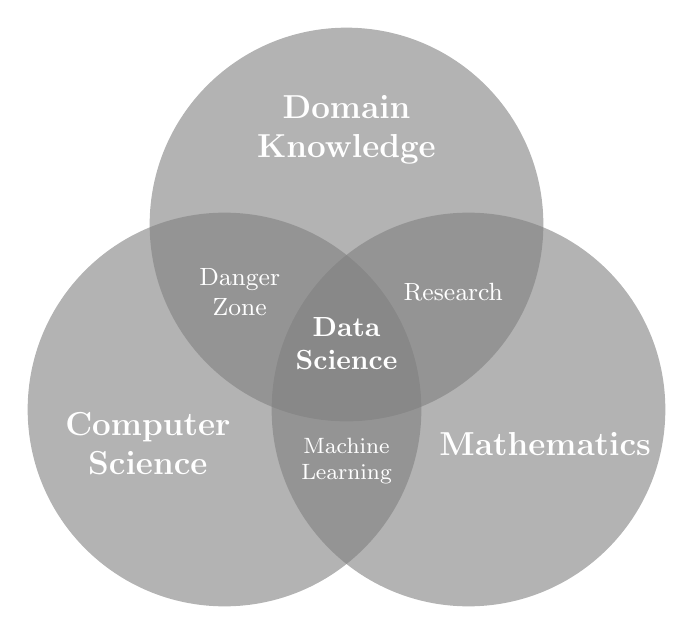
\begin{tikzpicture}[line join=bevel, line width=.7pt]
% Circles
\begin{scope}[on above layer]
\node[circle, minimum size=5cm, fill=gray, fill opacity=.6] (A) {};
\end{scope}
\node[circle, minimum size=5cm, fill=gray,fill opacity=.6, below left=-1.2cm and -2cm of A] (B) {};
\node[circle, minimum size=5cm, fill=gray,fill opacity=.6, below right=-1.2cm and -2cm of A] (C) {};
% Text
\begin{scope}[on above layer]
\node[yshift=-1.3cm, align=center, text=white, font=\large] at (A.north) {\textbf{Domain}\\\textbf{Knowledge}};
\node[xshift=1.5cm, align=center, text=white, font=\large] at (B.180+10) {\textbf{Computer}\\\textbf{Science}};
\node[xshift=-1.5cm, align=center, text=white, font=\large] at (C.-10) {\textbf{Mathematics}};

\node[xshift=1cm, align=center, text=white, font=\small] at (A.180+20) {Danger\\Zone};
\node[xshift=-1cm, align=center, text=white, font=\small] at (A.-20) {Research};
\node[yshift=-.5cm, align=center, text=white, font=\footnotesize] at (A.south) {Machine\\Learning};

\node[yshift=1cm, align=center, text=white, font=\normalsize] at (A.south) {\textbf{Data}\\\textbf{Science}};

\end{scope}

\end{tikzpicture}

\end{document}
